\documentclass[tikz,border=10pt]{standalone}
\usepackage{tikz}
\usetikzlibrary{arrows, positioning}

\begin{document}
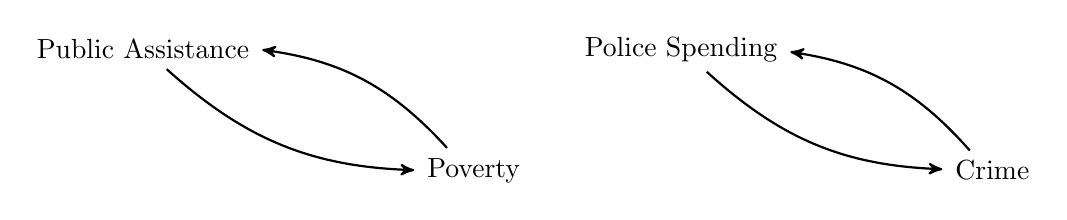
\begin{tikzpicture}[>=stealth',shorten >=1pt,auto,node distance=3cm, thick]

  % First diagram
  % Nodes
  \node (1) {Public Assistance};
  \node (2) [below right=1cm and 2cm of 1] {Poverty};

  % Edges
  \draw[->] (1) to[bend right=20] (2);
  \draw[->] (2) to[bend right=20] (1);

  % Second diagram
  % Nodes
  \node (3) [right=4cm of 1] {Police Spending};
  \node (4) [below right=1cm and 2cm of 3] {Crime};

  % Edges
  \draw[->] (3) to[bend right=20] (4);
  \draw[->] (4) to[bend right=20] (3);

\end{tikzpicture}
\end{document}
